\subsection{Distances}
\vspace{1cm}

Une tâche nécessaire à la mise en place de l’algorithme d’automatisation des désignations d’arbitres était de pouvoir quantifier la distance séparant les arbitres des gymnases. Cette donnée devait servir de critère lors de la sélection automatique, mais devait également être disponible directement sur l’interface. 

Les distances entre les arbitres et les gymnases devaient donc être stockées en base de données sous forme de matrice pour permettre de récupérer facilement une distance entre le domicile d’un arbitre et l’adresse d’un gymnase.
Face à ce problème, j’ai pensé à deux façon différentes de procéder : 
\begin{itemize}
    \item En créant une table unique associant une ligne par arbitre et une colonne par gymnase, l’intersection de chaque définissant une distance
    \item En stockant la matrice au format JSON dans une colonne de la table des arbitres, qui associe pour chaque arbitre l’id de chaque gymnase et sa distance avec celui-ci, puis effectue de façon symétrique cette étape dans la table des gymnases.
\end{itemize}

Le nombre d’arbitres et de gymnases étant évolutif et de l’ordre de plusieurs centaines, la deuxième option me paraissait plus facile à maintenir et à mettre en place.

\subsubsection{Coordonnées géographiques}
\vspace{1cm}

La première étape était de réfléchir à un moyen de récupérer les distances entre deux adresses. Pour ça deux méthodes s’offraient à moi :
\begin{itemize}
    \item La première était d’utiliser l’API Google Geocoding pour tous les arbitres et les gymnases. Cette API permet de récupérer les coordonnées GPS d’une adresse (longitude et latitude), ce qui pouvait me permettre de calculer la distance à vol d’oiseau séparant chaque arbitre et chaque gymnase grâce à une formule mathématique (Loi des cosinus).
    \item La deuxième méthode était d’utiliser l’API Google Matrix. Cette API permet de récupérer directement la matrice des distances entre une adresse de départ et plusieurs adresses d’arrivée.
\end{itemize}

Pour commencer, j’ai opté pour l’utilisation de la première méthode car celle-ci me permettait de réduire le nombre total de requêtes envoyées à Google.\\ 

En effet, cette méthode ne demandait qu’une requête par arbitre et par gymnase, ce qui équivalait pour $n$  arbitres et $m$ gymnases à un total de $n + m$  requêtes. La deuxième méthode demandait quant à elle un total de $n * m$ requêtes. Google n’autorise cependant qu’un nombre limité de requêtes gratuites par jour que je voulait éviter de dépasser.\\

La recherche de la formule mathématique permettant de calculer une distance entre deux points à partir de leurs coordonnées GPS a été faite sur des sites anglophones à cause du manque d’informations sur les sites francophones.

\newpage 

\begin{figure}
    \centering
    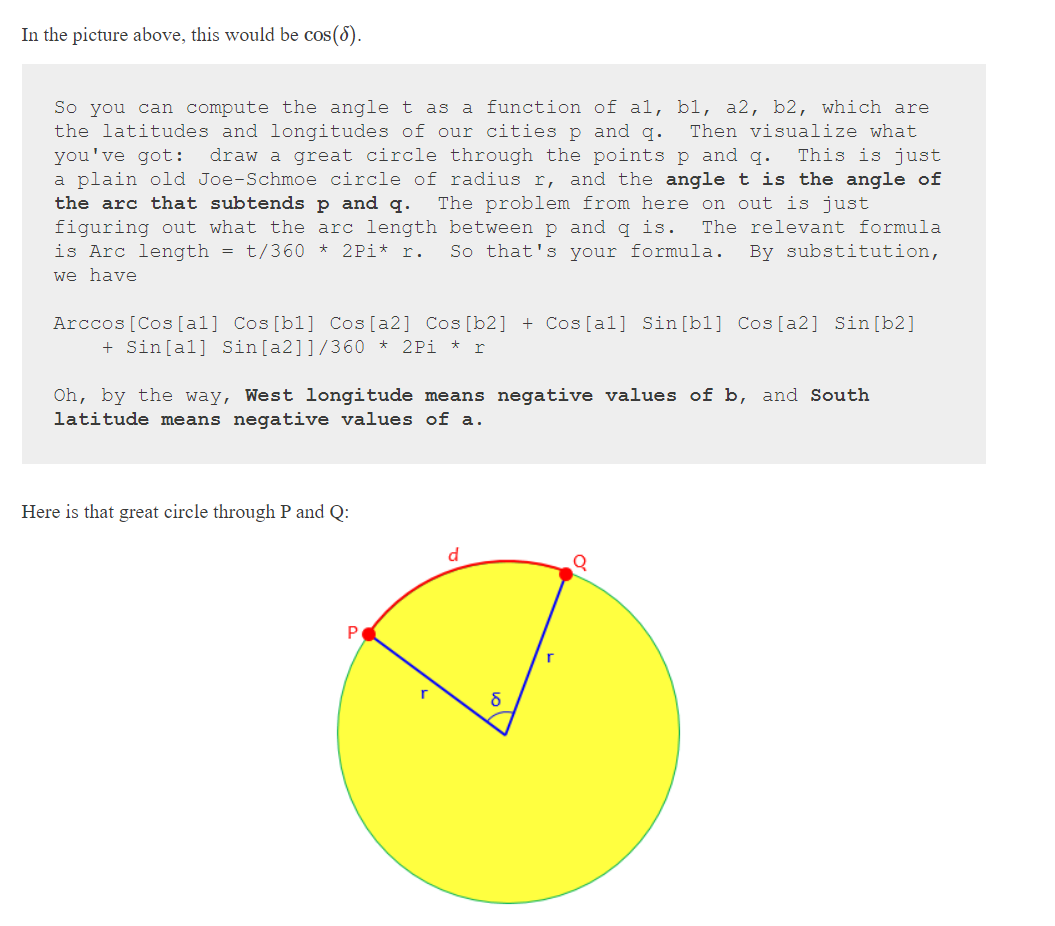
\includegraphics[width=\linewidth]{site_anglais.png}
    \caption{Article anglophone donnant une formulume pour calculer une distance à partir des coordonnées GPS}
\end{figure}

\begin{commentaire}
    Traduction : On peut calculer l’angle delta comme une fonction de paramètres a1, b1, a2 et b2 représentants respectivement les latitudes et longitudes des points P et Q. 
    Pour visualiser ce qu’on a : on dessine un cercle passant par nos points P et Q.
    Il s’agit simplement d’un cercle de rayon r, l’angle delta étant l’angle de l’arc qui relie les points P et Q. Le problème ici est de savoir quel est la distance de l’arc entre les points P et Q. La formule pertinente est : $d = \delta/360 * 2\pi * r$
\end{commentaire}

Pour effectuer le calcul de distance à partir de cette formule, j’ai mise en place un Trait possédant les méthodes nécessaires à la conversion de ces coordonnées en distances.

\begin{figure}[!h]
    \centering
    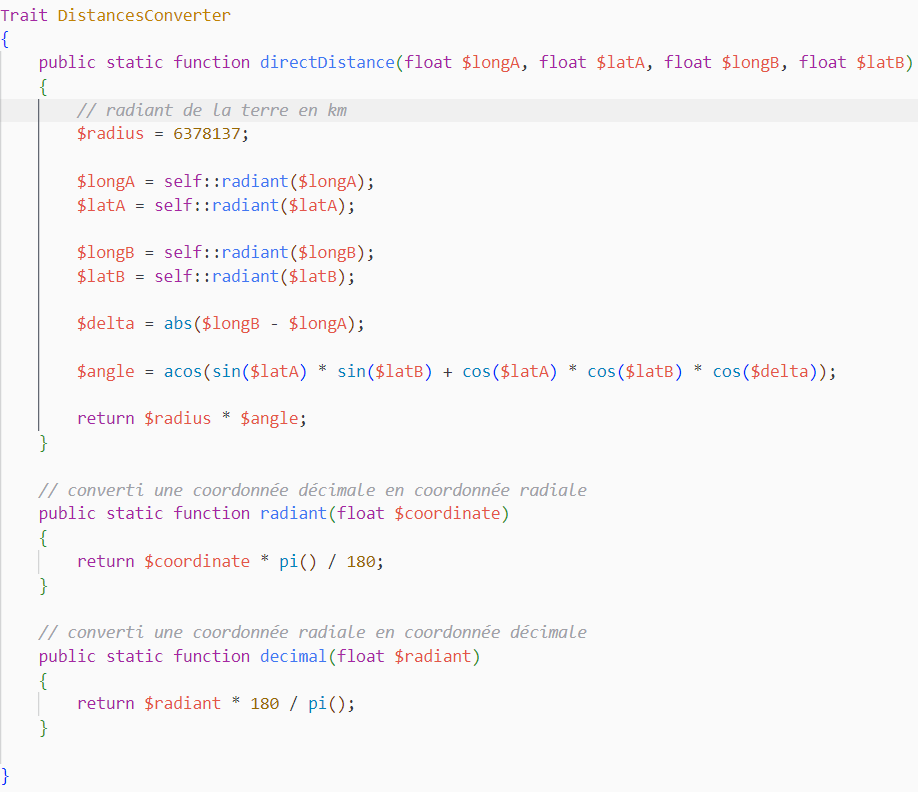
\includegraphics[width=\linewidth]{converter.png}
    \caption{Trait pour convertir des coordonnées GPS en distance}
\end{figure}

J’ai également mis en place les outils nécessaires à l’utilisation de la deuxième méthode pour l’utiliser à terme, car celle-ci permet la récupération d’informations plus riches et précises comme le temps de trajet en fonction du moyen de transport par exemple.

J’ai commencé par créer une classe avec deux méthodes distinctes pour effectuer les différentes requêtes.

\begin{figure}[!h]
    \centering
    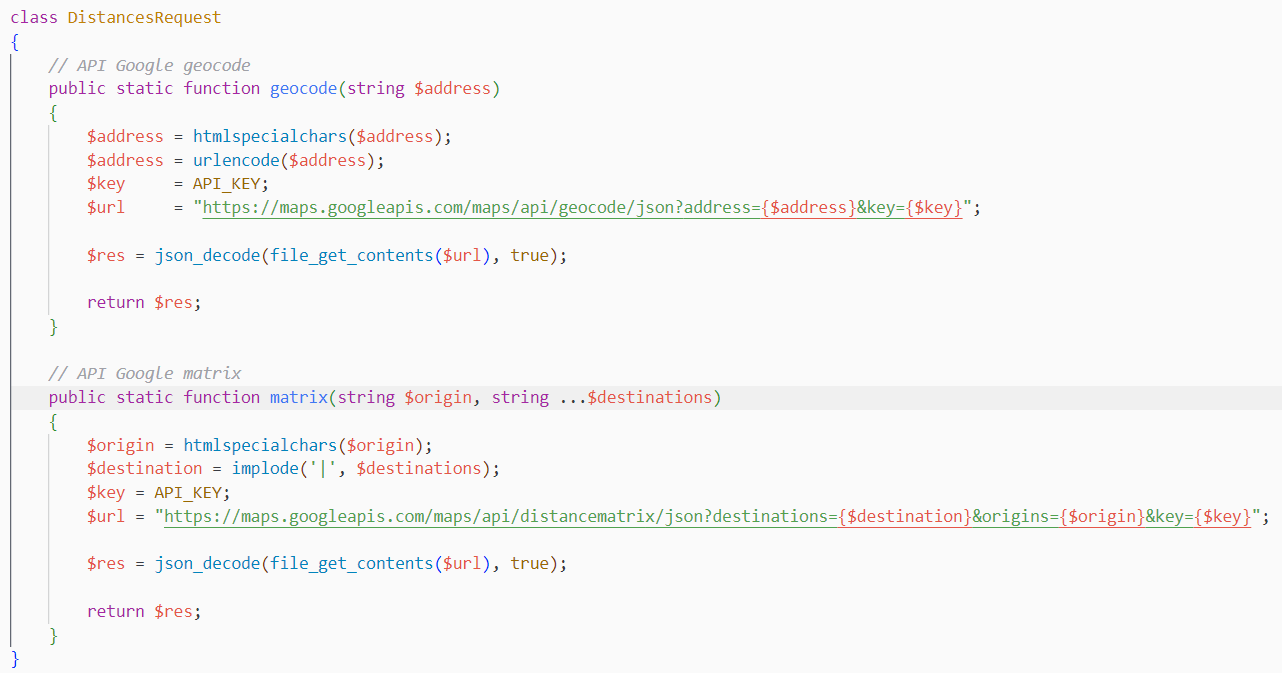
\includegraphics[width=\linewidth]{google.png}
    \caption{Composant pour envoyer des requêtes aux API Google}
\end{figure}

Les méthodes geocode et matrix récupèrent respectivement les réponses renvoyées par les API Google Geocoding et Google Matrix, sous forme de tableau associatif grâce à la fonction json\_decode pour une manipulation ultérieure.\\ \\

J’ai ensuite réalisé une classe pour la récupération et la mise en place des données géographiques dans la base de données. La récupération se base sur les méthodes de la classe \colored{DistanceRequest} , pour chaque arbitre et chaque gymnase disponibles dans la base de données (voir section sur la récupération des données).

La logique suivie par les méthodes de cette classe est d’abord de créer la colonne accueillant les coordonnées dans les tables si inexistante, puis d’insérer les coordonnées en se basant sur la réponse de l’API Google Geocoding.

À l’issu de ce processus, les tables des arbitres et des gymnases avaient toutes les deux une colonne supplémentaire avec les coordonnées géographiques de leur adresse. Ces coordonnées étaient sous format \colored{JSON} et stockaient \colored{null} si l’adresse était indisponible ou mal formatée.

\subsubsection{Matrice des distances}
\vspace{1cm}

Comme je l’ai expliqué dans l’introduction de ce chapitre, l’objectif avec ces coordonnées était de calculer la matrice des distances entre chaque adresse d’arbitre et de gymnase. 

Je me suis basé sur les outils du composant \colored{DistancesConverter} pour effectuer le calcul des distances, et j’ai ensuite stocké ces matrices sous forme de tableau associatif au format \colored{JSON} pour plus de flexibilité.

Ces matrices sont construites de façon à associer l’ID de chaque gymnase à la distance en mètres le séparant d’un arbitre, pour chaque arbitre puis de façon symétrique pour chaque gymnase.

Pour bien finir, et dans un objectif d’automatisation de ce processus dans le futur, j’ai finalement créé un composant dédié à la mise en place de ces matrices qui se base sur les classes de récupération de coordonnées et de calcul de distance à partir de celles-ci. 
Ce dernier appelle de façon procédurale les méthodes permettant de récupérer les coordonnées GPS et de calculer la matrice des distances pour chaque arbitre et chaque gymnase.